Los modelos de redes neuronales artificiales (ANN \textit{Artificial
Neural Network}), uno de los cuales es el
\textit{perceptrón} que discutiremos en este capítulo, están
inspirados en el cerebro humano.

Sin embargo, lo que busca la inteligencia artificial es construir
máquinas \textit{útiles} tomando como modelo el cerebro. El cerebro es
un dispositivo de procesamiento de información con habilidades
asombrosas que sobrepasan con creces a los más grandes esfuerzos de la
ingeniería en campos como son visión, aprendizaje y reconocimiento del habla,
por nombrar algunos.

\section{Inspiración en la biología}
El cerebro humano es muy diferente de una computadora. Mientras una
computadora tiene un número reducido de procesadores, el cerebro está
compuesto de una enorme cantidad (se estiman $10^{11}$) de unidades de
procesamiento llamadas \textbf{neuronas} trabajando en paralelo.

Aunque los detalles son inciertos, se cree que las neuronas son mucho
más simples y lentas que un procesador de una computadora
\cite{ethem}. Lo que hace al cerebro distinto, y le da su gran poder
computacional, es su gran conectividad: cada neurona en el cerebro
tienen conexiones, llamadas \textit{sinapsis}, con alrededor de otras
$10^{4}$ neuronas.

En una computadora, el procesador es activo y la memoria está separada
operando de forma pasiva (el procesador accede a ella sólo cuando se
requiere); se cree que en el cerebro, tanto el procesamiento como la
memoria están distribuidos por toda la red. El procesamiento es
efectuado por las neuronas y la memoria se encuentra en las sinapsis
entre ellas.

El cerebro es, además, un órgano capaz de adaptarse a las condiciones
de su ambiente, ya que constantemente son agregadas nuevas conexiones
sinápticas entre neuronas y modificadas las ya existentes. Una vez que
una neurona ha emitido una señal eléctrica, las adyacentes reciben la
información por medio de canales de transmisión llamados
\textit{dendritas}. Estos impulsos son llevados hasta la membrana
de la neurona para su procesamiento y, posteriormente, una reacción es
transmitida a través del \textit{axón} de la célula
\cite{memes}.
\begin{figure}[h]
  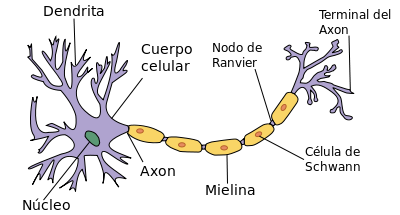
\includegraphics{neurona} \centering
  \caption{Estructura de una neurona. (Tomado de
    \url{https://es.wikipedia.org/wiki/Neurona})}
\end{figure}

\section{El perceptrón}
En 1943, Warren McCullock y Walter Pitts publican la primera
aproximación de una neurona simplificada, tratando de entender cómo
funciona el cerebro biológico para el diseño de inteligencia
artificial, la llamada neurona McCullock-Pits (MCP) \cite{mcp}.

McCullock y Pitts describen a la neurona como una compuerta lógica
sencilla con una salida binaria; múltiples señales llegan a las
dendritas para ser integradas al cuerpo de la célula. Si la señal
acumulada excede cierto umbral, se genera una señal de salida que se
le pasa al axón.

Unos años después, Frank Rosenblatt publicó la primera aproximación al
concepto de perceptron basado en el modelo de neuronas MCP
\cite{rosenblatt}. Intuitivamente, el algoritmo aprende
automáticamente los coeficientes de pesos óptimos que luego se
multiplican con las características de entrada para tomar la decisión
de si la neurona se activa o no. Este algoritmo podría ser usado
entonces para predecir si una muestra pertenece a una clase o a otra
\cite{python}.

Formalmente, podemos plantearlo como un problema de clasificación
binaria, donde nos referimos a nuestras dos clases, por simplicidad,
como 1 (clase positiva) y -1 (clase negativa). Definimos también una
\textit{función de activación $\mathbf{\phi (z)}$} que toma una
combinación lineal de ciertos valores de entrada \textbf{x} y un
vector de pesos \textbf{w}, donde \textbf{z} es lo que llamamos
\textit{entrada de la red} $(z = w_1x_1 + ... + w_mx_m)$:

\begin{equation*}
w=
    \begin{bmatrix}
        w_1 \\ \vdots \\ w_m
    \end{bmatrix}
    , x=
    \begin{bmatrix}
      x_1 \\ \vdots \\ x_m
    \end{bmatrix}
\end{equation*}
\\ Si la activación de una muestra particular $x^{(i)}$ es mayor que
un parámetro definido $\theta$, predecimos la clase 1, y la clase -1
en caso contrario. En el algoritmo del perceptrón de Rosenblatt, la
función de activación $\phi$ es una \textit{función escalón},
que es llamada a veces la \textit{función de Heaviside}:
\begin{equation*}
  \phi(z)= \left\{ \begin{array} {rl} 1 & \text{si } z \geq \theta
    \\ -1 & \text{en otro caso} \end{array} \right.
\end{equation*}

Por simplicidad, definimos $w_0=-\theta$ y $x_0=1$, escribiendo
entonces a $z$ de la forma $z=-\theta + w_1x_1 + \dots + w_mx_m =
\mathbf{w^Tx}$.  La figura \ref{fig:binary} ilustra cómo la entrada de
la red $z=w^Tx$ es \textit{aplanada} a una salida binaria (-1 o 1) por
la función de activación del perceptrón (izquierda) y cómo puede ser
usada para discriminar entre dos clases linealmente separables
(derecha):
\begin{figure}[H]
  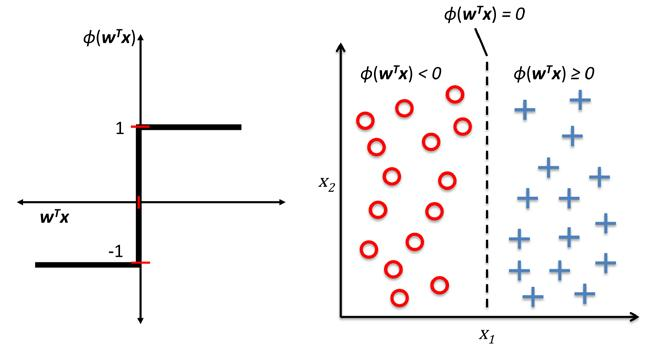
\includegraphics[scale=0.5]{perceptron} \centering
  \caption{\textit{Aplanamiento} de la salida del perceptrón para
    hacer clasificación.  (Tomado de \cite{python})}
  \label{fig:binary}
\end{figure}

La idea detrás del modelo de perceptron de Rosenblatt es reducir a una
abstracción de cómo funciona una neurona: se activa o no se
activa. Así, la regla inicial de Roseblatt es relativamente simple y
puede ser resumida en los siguientes pasos:
\begin{enumerate}
  \item Inicializar los pesos en cero o en números aleatorios cercanos
    a cero.
  \item Para cada muestra de entrenamiento $x^{(i)}$ realizar los
    siguientes pasos:
  \begin{enumerate}
    \item Calcular el valor de salida $\hat y$.
    \item Actualizar los pesos en $w$.
  \end{enumerate}
\end{enumerate}


En este caso, el valor de salida es la clasificación dada por la
función escalón definida previamente (\textit{i.e.} $\hat y
= \phi(z)$) y la actualización simultánea de cada peso $w_j$ en el
vector de pesos $w$ puede ser escrito más formalmente como:
\begin{equation}
  w_j := w_j + \Delta w_j
\end{equation}

El valor de $\Delta w_j$, que es usado para actualizar el peso $w_j$,
es calculado por la regla de aprendizaje del perceptrón:
\begin{equation}
  \Delta w_j = \eta (y^{(i)} - \hat y^{(i)})x^{(i)}_j
\end{equation}

Donde $\eta$ es el índice de aprendizaje (una constante entre 0 y 1),
$y^{(i)}$ es la clasificación real de la i-ésima muestra, y $\hat
y^{(i)}$ es la clasificación dada por la predicción. Es importante
recalcar que todos los pesos en el vector de pesos son actualizados de
manera simultánea, lo que significa que no recalculamos $\hat y^{(i)}$
hasta que todos los pesos $\Delta w_j$ han sido actualizados.

\begin{figure}[H]
  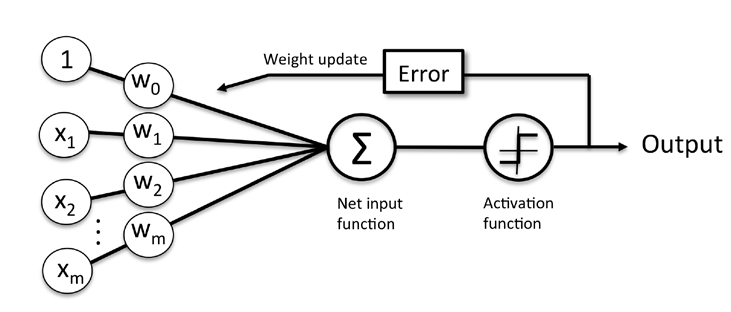
\includegraphics[scale=0.5]{perceptron-summary} \centering
  \caption{Resumen del concepto general de perceptrón. (Tomado de
    \cite{python})}
  \label{fig:perceptron}
\end{figure}

La figura \ref{fig:perceptron} muestra cómo el perceptrón recibe las
entradas de una muestra $x$ y las combina con los pesos $w$ para
calcular la entrada neta.  Esta entrada se le da a la función de
activación, que genera una salida binaria (-1 o 1 en este caso),
representando la predicción de la clasifica- ción. Durante la fase de
aprendizaje, la salida es usada para calcular el error de la
predicción y actualizar los pesos.

\section{Neuronas adaptativas lineales}

\begin{figure}[H]
  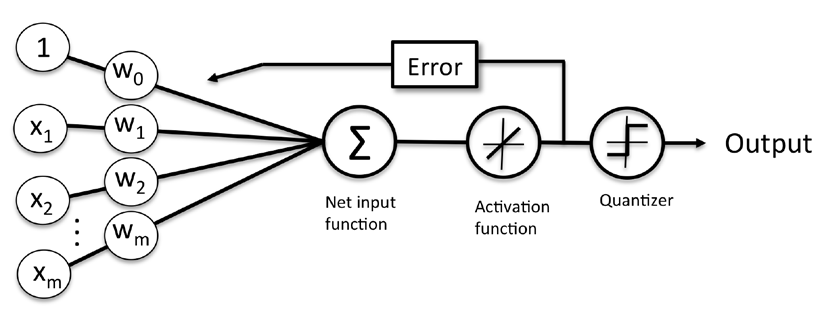
\includegraphics[scale=0.5]{adaline} \centering
  \caption{Esquema de Adaline. (Tomado de \cite{python})}
  \label{fig:adaline}
\end{figure}

La neurona adaptativa lineal (\textbf{Adaline}) fue publicada por
Bernard Widrow \cite{adaline} unos años después del algoritmo del
perceptrón de Frank Rosenblatt, y se le considera su evolución natural.

El algoritmo de Adaline es particularmente interesante porque ilustra
el concepto clave de definir y minimizar funciones de costo, lo que
sienta las bases para algoritmos más avanzados de clasificación, como
la regresión logística o las máquinas de vectores de apoyo.

La principal diferencia entre las reglas de Adaline (también llamada
de \textit{Widrow-Hoff}) y la del perceptrón de Rosenblatt es que los
pesos son actualizados con base en una función de activación lineal,
en lugar de una función escalón. En Adaline, esta función de
activación $\phi (z)$ es simplemente la función identidad de la
entrada neta, así $\phi (w^T x) = w^T x$.

Mientras que la función de activación lineal es usada para la
actualiza- ción de pesos, un \textit{cuantificador}, similar a la
función escalón descrita anteriormente, puede ser usado para hacer la
clasificación, como se ilustra en la figura \ref{fig:adaline}.

Si se comparan las figuras \ref{fig:perceptron} y
\ref{fig:adaline}, la diferencia es que se usa la salida con valores
continuos de la función lineal de activación para calcular el error y
actualizar los pesos, en lugar de hacer una clasificación binaria.

Cabe destacar que actualmente se buscan funciones de activación con
curvas más suavizadas y, sobre todo, diferenciables. Esto con el fin
de optimizar los parámetros de los modelos más complejos.

\begin{center}
\begin{figure}[H]
  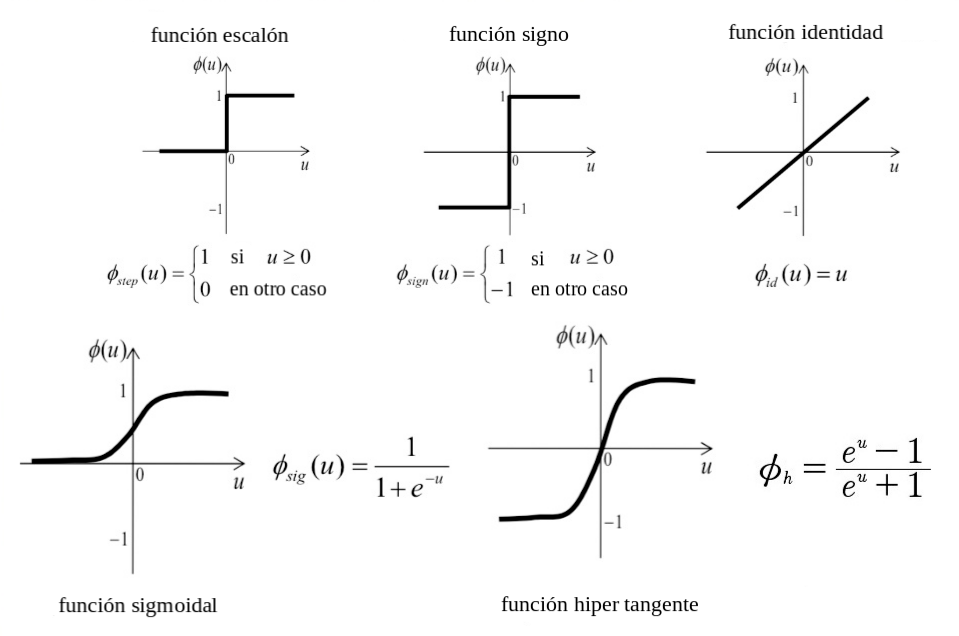
\includegraphics[scale=0.5, center]{activation} \centering
  \caption{Algunos ejemplos de otras funciones de activación.  (Tomado
    de
    \url{https://www.slideshare.net/SungJuKim2/multi-layer-perceptron-back-propagation})}
\end{figure}
\end{center}

\section{El perceptrón multicapa}
El perceptrón multicapa es una generalización del perceptrón simple de
Rosenblatt, como consecuencia de las limitaciones de éste ante
conjuntos de datos que no son linealmente separables. Lo que se hace
es combinar varios perceptrones en una \textit{red neuronal de
propagación hacia adelante}, con una estructura
de \textit{capas}\footnote{Entendiendo \textit{capa} como perceptrones
en paralelo, donde están conectados de cada lado a las capas
adyacentes, formando así una especie de \textit{red}}.

La información fluye de capa en capa en el mismo sentido, desde la
\textit{capa de entrada} donde están los datos sin procesar, hasta la
\textit{capa de salida} donde se da la clasificación. Cada una de las capas
intermedias, llamadas \textit{capas ocultas}, consta de un conjunto de
neuronas sin conexiones entre ellas, pero totalmente conectadas a las
capas inmediatamente anterior y posterior. Visto como una gráfica, un
\textbf{perceptrón multicapa} (MLP, \textit{Multilayer Perceptron})
es una gráfica $n$-partita dirigida donde $n$ sería el número de
capas.
\begin{figure}[H]
  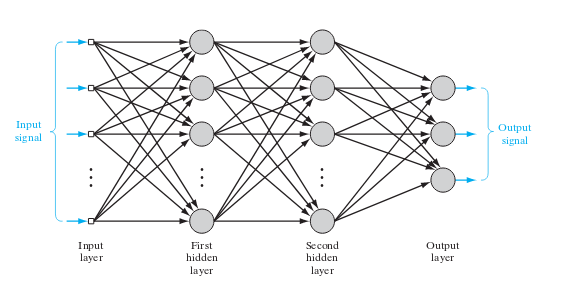
\includegraphics[scale=1.3]{mlp} \centering \caption{Arquitectura de
  un MLP con una capa oculta (Tomado de \url{https://es.wikipedia.org/wiki/Perceptron_multicapa})}
\end{figure}
Cada neurona oculta actua como un \textit{detector de
  características}. Conforme va avanzando el proceso de aprendizaje,
las neuronas ocultas comienzan a ``descubrir'' gradualmente las
características más sobresalientes de los datos de entrenamiento.
Esto se logra a través de una serie de transformaciones no lineales,
dadas por las funciones de activación y pesos específicos de cada
neurona.

Inicialmente, a cada conexión se le asigna un peso aleatorio. Dada la
estructura en capas de la red, es mucho más fácil visualizar y
manipular estos pesos acomodandolos en una matriz $W$, que llamaremos
\textit{matriz de pesos}, donde $W_i$ son los pesos de la $i$-ésima
capa de la red. Entonces, dado un vector de entrada $x$, la primera
capa oculta $h_1$ calcula su valor a partir de $W_1$ y una traslación
$b_1$, que llamamos \textit{sesgo} (\textit{bias}, inglés), del
siguiente modo:
\begin{equation}
  h_1 = \phi(W_1x + b_1)
\end{equation}
donde $\phi$ es una función de activación no lineal y
diferenciable. Así la $i+1$-ésima capa oculta computa su valor como
\begin{equation}
  h_{i+1} = \phi(W_{i+1}h_i + b_{i+1})
\end{equation}
Por último, la salida, suponiendo que hay $n$ capas ocultas, sería
\begin{equation}
  \hat{y} = \phi{(W_{n+1}h_n + b_{n+1})}
\end{equation}
donde $\hat{y}$ es el vector de clasificación.

\section{Descenso por el gradiente}
Uno de los puntos clave del aprendizaje de máquina supervisado es
definir una función objetivo que deberá ser optimizada durante el
proceso de aprendizaje. Esta función objetivo usualmente es una
\textbf{función de costo, pérdida o error} que se quiere minimizar.

Definimos la función de costo $J$ como la \textbf{Suma de los errores
  cuadrados} (SSE, \textit{Squared Sum Error}) entre la salida
  calculada y el valor real.
\begin{equation}
  J(w)=1/2n \sum_i (\hat{y}_i - y_i^2)
\end{equation}
donde $w$ es el conjunto de los parámteros de la red, es decir
$w:=\bigcup{W_i, b_i}_{i=1}^{n}$, $n$ el número de capas de la red, y
$y_i$ la $i$-ésima etiqueta de entrenamiento. La principal ventaja de
esta función de error, además de ser lineal es que la función de
costos se vuelve diferenciable.

La no-linealidad de las funciones de activación provoca que no se
garantice la convexidad de las funciones de error más comunes, es
decir, que no existe un método analítico para encontrar el mínimo de
la función de error. El entrenamiento de la red se basa en métodos
iterativos que van reduciendo paulatinamente ese error.

Sabemos que la derivada es útil para minimizar funciones porque, dada
una función $y = f(x)$, nos dice cómo cambiar $x$ para hacer una
pequeña mejora en $y$, en otras palabras $f(x-\varepsilon f'(x)) <
f(x)$ para un $\varepsilon \in \mathbb{R}$ suficientemente
pequeño. Podemos entonces minimizar $f(x)$ al mover a $x$ en pequeños
\textit{pasos} con el signo opuesto de la derivada. A esta técnica se
le conoce como \textbf{descenso por el gradiente}\footnote{Puede
pensarse en el gradiente como una generalización de la derivada para
espacios $n$-dimensionales}.

La idea detrás del descenso por el gradiente es disminuir el gradiente hasta encontrar
un mínimo (local o global) de la función de costo. En cada iteración, se reduce
un \textit{paso} del gradiente, donde cada \textit{paso} está determinado por
el valor del índice de aprendizaje, así como por la pendiente del gradiente.

\begin{figure}[H]
\begin{center}
  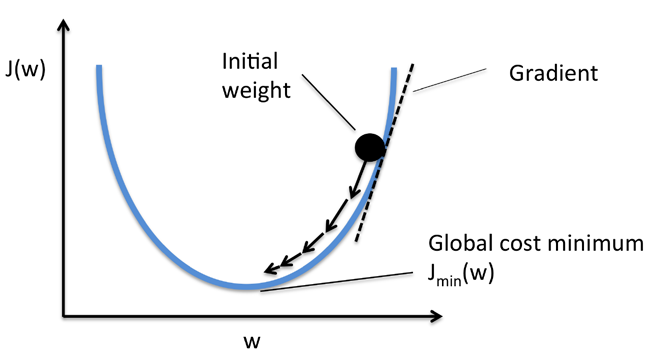
\includegraphics[scale=0.5]{gradient-descent}
  \caption{Diagrama de descenso por el gradiente. (Tomado de \cite{python})}
\end{center}
\end{figure}

Usando el descenso por el gradiente, se pueden actualizar los pesos quitandole un \textit{paso}
al gradiente $\nabla J(w)$ de la función de costos $J(w)$:
\begin{equation}
  w:=w + \Delta w
\end{equation}

En donde el cambio de peso $\Delta w$ se define como el gradiente negativo multiplicado
por el índice de aprendizaje $\eta$:
\begin{equation}
  \Delta w:=-\eta \Delta J(w)
\end{equation}

Calculamos la derivada parcial de la función de costos SSE con respecto al
j-ésimo peso de la siguiente manera:
\begin{equation*}
\begin{split}
  \frac{\partial J}{\partial w_j} &= \frac{\partial}{\partial w_j}\frac{1}{2}\sum_{i=1}^n (y^{(i)} - \phi(z^{(i)}))^2 \\
  &= \frac{1}{2}\sum_{i=1}^n 2(y^{(i)} - \phi(z^{(i)}))\frac{\partial}{\partial w_j}(y^{(i)} - \phi(z^{(i)}))\\
  &= \sum_{i=1}^n (y^{(i)} - \phi(z^{(i)}))\frac{\partial}{\partial w_j}(y^{(i)} - \phi (z^{(i)}))\\
  &= \sum_{i=1}^n(y^{(i)} - \phi(z^{(i)}))(-x_j^{(i)})\\
  &= -\sum_{i=1}^n(y^{(i)} - \phi(z^{(i)}))x_j^{(i)}
\end{split}
\end{equation*}

\section{Descenso estocástico por el gradiente}
Si se considera el caso en el que se tiene un conjunto de datos con
millones de puntos con datos, correr un entrenamiento con descenso por
el gradiente puede ser un proceso sumamente costoso computacionalmente
ya que se requiere reevaluar todo el conjunto de datos cada vez que se
toma un \textit{paso} hacia el mínimo global.

Una alternativa popular al algoritmo de descenso por el gradiente es el
\textbf{descenso estocástico por el gradiente}, llamado también
descenso por el gradiente iterativo. En lugar de actualizar los pesos
basado en la suma de los errores acumulados de todas las muestras
$x^{(i)}$:
\begin{equation}
  \Delta w = \eta \sum_i(y^{(i)} - \phi(z^{(i)}))x^{(i)}
\end{equation}

se actualizan los datos de manera incremental para cada muestra del
entrenamiento:
\begin{equation}
  \Delta w = \eta(y^{(i)} - \phi(z^{(i)}))x^{(i)}
\end{equation}

Aunque el descenso estocástico por el gradiente podría ser considerado
una aproximación del descenso por el gradiente, por lo general
converge mucho más rápido debido a las actualizaciones más frecuentes
de los pesos. Como cada gradiente se calcula basado en un sólo ejemplo
de entrenamiento, el error tiende a tener más entropía, lo que
permite que el descenso estocástico por el gradiente
pueda \textit{escapar} más fácilmente de un mínimo local. Para obtener
buenos resultados con el descenso estocástico por el gradiente es
importante que se tomen los datos de forma aleatoria.

Otra ventaja del descenso estocástico por el gradiente es que se puede
usar para hacer \textit{aprendizaje en línea}. Esto quiere decir que
el modelo es entrenado al momento, mientras más y más datos van
llegando. Esto es especialmente útil cuando se están acumulando
grandes cantidades de datos.  Usando entrenamiento en línea, el
sistema puede adaptarse inmediatamente a los cambios y los datos de
entrenamiento pueden ser descartados después de actualizar el modelo,
si el espacio de almacenamiento fuera un problema.

Las redes neuronales son modelos complejos que por lo general tienen
un alto número de mínimos locales, volviendo al descenso por el
gradiente poco efectivo como mecanismo de entrenamiento, incluso
utilizando la variante estocástica. Sin embargo, redes altamente
eficientes usualmente son entrenadas utilizando descenso por el
gradiente. ¿Cómo explicar esta aparente contradicción?

Recientemente, evidencia empírica \cite{choromanska} ha dado indicios
de que las ANN tienen la mayoría de sus mínimos locales cerca del
mínimo global. Esto quiere decir que \textbf{el descenso por el
gradiente estocástico funciona ``suficientemente bien''}, ya que
puede \textit{escapar} de los mínimos locales sin alejarse demasiado
del mínimo global. Hay otros métodos más avanzados que son empleados
para entrenar ANNs, pero en este trabajo utilizamos descenso por el
gradiente por su simplicidad e interpetación tan intuitiva.

\section{Retropropagación}
Para utilizar de forma efectiva el descenso por el gradiente, es
necesario una forma eficiente de computar el gradiente de una función
de error. La propagación hacia atrás o retropropagación
(\textit{Backpropagation}) nos permite hacerlo.

Definimos para cada neurona $j$ en la capa $l$ la salida $o^{(l)}_j$ como
\begin{equation}
\label{eqn:def_o}
  o^{(l)}_j = \phi(a^{(l)}_j) = \phi(\sum_{k=1}^n w_{kj}o_k^{(l-1)})
\end{equation}
donde $\phi$ es la función de activación y $a_j^{(l)}$ se refiere a la
suma de los pesos de las salidas de las neuronas de la capa inmediata
anterior. Comunmente, llamamos a $a_j^{(l)}$ la \textit{activación} de
la neurona.

Supongamos ahora que queremos encontrar la derivada parcial de la
función de errir con respecto a $w_{ij}$.
Para encontrar cómo cambia una función de error $J$ cambia con respecto
al peso $w_{ij}$, aplicamos la regla de la cadena:
\begin{equation}
  \frac{\partial J}{\partial w_{ij}} = \frac{\partial J}{\partial o_j^{(l)}}
  \frac{\partial o_j^{(l)}}{\partial a_j^{(l)}} \frac{\partial a_j^{(l)}}{\partial w_{ij}}
\end{equation}

A partir de \ref{eqn:def_o}, podemos ver que
$a_j^{(l)} = \sum_{k=1}^n w_{kj}o_k^{(l-1)}$. Esto implica que
$\frac{\partial a_j^{(l)}}{\partial w_{ij}} = o_i^{(l-1)}$. Definimos entonces
\begin{equation}
  \delta_j^{(l)} = \frac{\partial J}{\partial o_j^{(l)}} \frac{\partial o_j^{(l)}}{a_j^{(l)}}
\end{equation}

Así, tenemos que
\begin{equation}
  \frac{\partial J}{\partial w_{ij}} = \delta_j^{(l)}o_i^{(l-1)}
\end{equation}
Resulta entonces que tenemos una identidad recursiva para
$\delta_j^{(l)}$, llamada la fórmula de la retropropagación
\begin{equation}
  \delta_j^{(l)} = \phi'(a_j^{(l)})\sum_m w_{jm} d_m^{(l+1)}
\end{equation}
donde la suma es sobre las neuronas conectadas a la $j$-ésima neurona
de la capa $l$.

Podemos entonces derivar esta identidad utilizando la regla de la cadena
para escribir $\frac{\partial J}{\partial o_j^{(l)}}$ en términos de
$\frac{\partial J}{\partial a_m^{(l+1)}}$ y $\frac{\partial a_m^{(l+1)}}{\partial o_j^{(l)}}$.

\begin{equation}
\begin{split}
  \delta_j^{(l)} &= \frac{\partial J}{\partial o_j^{(l)}} \frac{\partial o_j^{(l)}}{\partial a_j^{(l)}} \\
  &= \frac{\partial o_j^{(l)}}{\partial a_j^{(l)}} \frac{\partial J}{\partial o_j^{(l)}} \\
  &= \phi' (a_j^{(l)}) \sum_m \frac{\partial J}{\partial o_m^{(l+1)}} \frac{\partial o_m^{(l+1)}}{\partial a_m^{(l+1)}} \frac{\partial a_m^{(l+1)}}{\partial o_j^{(l)}} \\
  &= \phi'(a_j^{(l)}) \sum_m \delta_m^{(l+1)}w_{jm}
\end{split}
\end{equation}

Notemos que esto nos permite computar capas anteriores a $\delta_j$ a
través de las capas posteriores, de ahí el nombre de retropropagación.
Podemos computar $\delta_j$ directamente, si $j$ es una capa de salida,
así que este proceso eventualmente termina.
